\documentclass[11pt]{article}
\usepackage{acl2014}
\usepackage{times}
\usepackage{url}
\usepackage{latexsym}
\usepackage{hyperref}
\usepackage{graphicx}

\title{Name of your project}

\author{Sergio Kazatzidis \\
    {\tt sergio@example.com} \\
    Kamiel Fokkink \\
    {\tt kamielfokkink@gmail.com} \\\And
    Baran İşcanlı \\
    {\tt barantevitol@gmail.com} \\
    Tomas Kehus \\
    {\tt tekehus@gmail.com}}

\date{}

\begin{document}
\maketitle
\begin{abstract}
    Recommender systems are used to predict recommendations for a user based on previous behaviour, that will match the users preferences and interests. They are widely popular in the consumer service industry, and they work well to give a personalized advice to customers. The goal of this project is to build two recommender systems, based on two common approaches: user based and content based recommendations. The machine learning principle behind these models is k Nearest Neighbours, which looks at the k most similar datapoints to a target point.
\end{abstract}

\noindent

\section{Introduction}
Recommender systems are a set of techniques to recommend new products to a user, and are widely used in industries that provide consumer products. Netflix uses it to recommend movies to its users, Facebook uses it to build up a newsfeed, and Youtube recommends videos that its users might want to view. The algorithm tries to predict recommendations for users that are likely to match their needs or interests, based on their previous purchasing or viewing patterns. They rely on large amounts of data that track patterns in peoples' behaviour, to build up a profile of the user, and be able to predict a meaningful recommendation. There are two main ways to approach this problem. Collaborative filtering looks at relationships and similarities between users, and content based filtering looks at relationships between items. Many industrial implementations make use of a hybrid version that combines elements of the two. Our goal for this project is to create recommender systems for amazon customers, based on their previous purchases and ratings. It will build a model for the two types of recommendations, those based on user-to-user, and item-to-item. \\

\section{Dataset}
The dataset that we used for the training of our model was Amazon review data, which was retrieved from \href{http://jmcauley.ucsd.edu/data/amazon/}{here}. This database contains review information about numerous kinds of products, ranging from groceries to clothes to video games. But reviews about for example kitchen appliances would say more about the quality of the product, and not about a consumers individual tastes. The most suitable kinds of products to train a recommender system on are those of which the review reflects the particular persons interests and tastes. Therefore, we chose to use the datasets of Kindle books, video games, and digital music. The database offers two options for the dataset: all aggregated reviews, or a filtered dataset to only include reviewers that rated 5 or more products. We chose the second option, because it reduces the cost of training, and it is more relevant to have several datapoints per user, so as to have more information for good recommendations. \\

\subsection{Splitting the data}
The sizes of the datasets are: 31MB and 64k lines for the music, 110MB and 231k lines for the video games, and 266MB and 982k lines for the books. For each review, there are several features that we can include. Some are necessary for our analysis, such as the reviewer ID, product ID, and the review score. Many features are also less relevant for our purposes, but can be included if needed, such as the review time or a review text. A printout sample of the data can be seen in figure 1. \\
\begin{figure}
    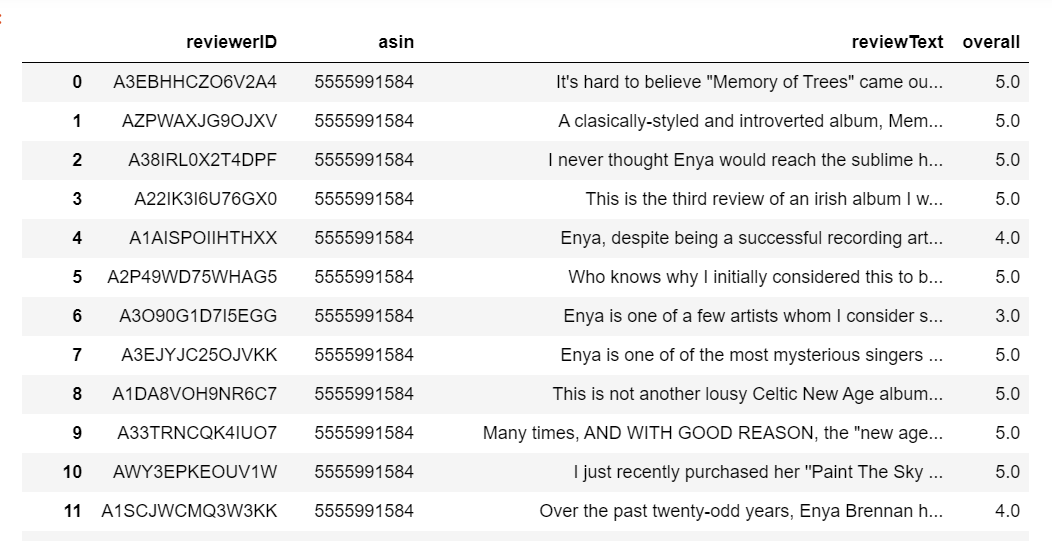
\includegraphics[width=10cm]{Pandas_df_example.png}
    \caption{Pandas dataframe of the data}
\end{figure}

For testing purposes, we want to split our data into a training and a testing set. This is not just a simple randomized split of the datapoints. For the evaluation of our recommender system, we need to split our user base, taking out 10\% of all users and putting them in a test set. Our test set will therefore consist of completely new users who have not been used for the training of our model. By looking at a few of those new user's preferences, the model can then recommend them new items to buy. We will be able to compare these recommendations to our expected recommendations, to evaluate our model.

\section{k-NN}
K-nn classification is a simple concept, where a point is given the same class as the nearest k points around it. The value of k is a hyperparameter, which has to be provided beforehand. In our case, we will try out different values for k, to find out which one has the optimal performance. K-nn has the advantages of speed and minimal necessary processing power. It also requires no training time- this can potentially be seen as a negative aspect, as there is no 'learning' within a model. However, our dataset has enough datapoints that it should be able to provide reliable recommendations, even with such a simple algorithm.\\
To compute the similarity between two users, we look at the intersection of shared rated items between the two users. This is approach is recommended by \footnote[1]{https://towardsdatascience.com/introduction-to-recommender-systems-6c66cf15ada}, as our data is sparse, and most items will not have been rated by both users. From the intersection of shared items, we compute the similarity between the two users' ratings of those items. However, just this similarity is not enough, it needs to be weighted. If a target user made twenty reviews, and shares just one item with another user, for which they gave the same rating, it would give a similarity of 1. This is obviously not the case, as the target user has rated 19 other items as well. Therefore, we weight the similarity with the length of the set of shared items, divided by the total amount of items rated by the target user.

\subsection{Similarity measures}
There are several ways to calculate the similarity between two users. A user is represented by a vector, where each entry is the users interaction with a product. These vectors are sparse, with most of the entries set to 0, as the user does not interact with most of the items. The other entries contain the users rating for that product, between 1 to 5. There are three similarity measures that we consider, and during the development phase we see which of these measures performs best. The first is Euclidean similarity, which is the inverse of the Euclidean distance of the points in space. The second is cosine similarity, which is the dot product of the two vectors scaled by their length, thus giving the angle between the vectors. The third is pearson correlation, a measure of the strength of linear dependence between two vectors. Because we only computed the similarity between the shared items, we need to weigh this similarity. If two users would have one item in common for which they both gave a 5.0, their similarity would be 1.0, but indeed they are quite different in their preferences. So we weigh the similarity by multiplying it with the size of their shared items divided by the amount of items reviewed by the target user.

\end{document}
